\documentclass[]{article}
\usepackage{lmodern}
\usepackage{amssymb,amsmath}
\usepackage{ifxetex,ifluatex}
\usepackage{fixltx2e} % provides \textsubscript
\ifnum 0\ifxetex 1\fi\ifluatex 1\fi=0 % if pdftex
  \usepackage[T1]{fontenc}
  \usepackage[utf8]{inputenc}
\else % if luatex or xelatex
  \ifxetex
    \usepackage{mathspec}
  \else
    \usepackage{fontspec}
  \fi
  \defaultfontfeatures{Ligatures=TeX,Scale=MatchLowercase}
\fi
% use upquote if available, for straight quotes in verbatim environments
\IfFileExists{upquote.sty}{\usepackage{upquote}}{}
% use microtype if available
\IfFileExists{microtype.sty}{%
\usepackage{microtype}
\UseMicrotypeSet[protrusion]{basicmath} % disable protrusion for tt fonts
}{}
\usepackage[margin=1in]{geometry}
\usepackage{hyperref}
\hypersetup{unicode=true,
            pdftitle={Índice de Actividad Económica Metropolitano},
            pdfauthor={DS @ OPI},
            pdfborder={0 0 0},
            breaklinks=true}
\urlstyle{same}  % don't use monospace font for urls
\usepackage{graphicx,grffile}
\makeatletter
\def\maxwidth{\ifdim\Gin@nat@width>\linewidth\linewidth\else\Gin@nat@width\fi}
\def\maxheight{\ifdim\Gin@nat@height>\textheight\textheight\else\Gin@nat@height\fi}
\makeatother
% Scale images if necessary, so that they will not overflow the page
% margins by default, and it is still possible to overwrite the defaults
% using explicit options in \includegraphics[width, height, ...]{}
\setkeys{Gin}{width=\maxwidth,height=\maxheight,keepaspectratio}
\IfFileExists{parskip.sty}{%
\usepackage{parskip}
}{% else
\setlength{\parindent}{0pt}
\setlength{\parskip}{6pt plus 2pt minus 1pt}
}
\setlength{\emergencystretch}{3em}  % prevent overfull lines
\providecommand{\tightlist}{%
  \setlength{\itemsep}{0pt}\setlength{\parskip}{0pt}}
\setcounter{secnumdepth}{0}
% Redefines (sub)paragraphs to behave more like sections
\ifx\paragraph\undefined\else
\let\oldparagraph\paragraph
\renewcommand{\paragraph}[1]{\oldparagraph{#1}\mbox{}}
\fi
\ifx\subparagraph\undefined\else
\let\oldsubparagraph\subparagraph
\renewcommand{\subparagraph}[1]{\oldsubparagraph{#1}\mbox{}}
\fi

%%% Use protect on footnotes to avoid problems with footnotes in titles
\let\rmarkdownfootnote\footnote%
\def\footnote{\protect\rmarkdownfootnote}

%%% Change title format to be more compact
\usepackage{titling}

% Create subtitle command for use in maketitle
\newcommand{\subtitle}[1]{
  \posttitle{
    \begin{center}\large#1\end{center}
    }
}

\setlength{\droptitle}{-2em}
  \title{Índice de Actividad Económica Metropolitano}
  \pretitle{\vspace{\droptitle}\centering\huge}
  \posttitle{\par}
  \author{DS @ OPI}
  \preauthor{\centering\large\emph}
  \postauthor{\par}
  \predate{\centering\large\emph}
  \postdate{\par}
  \date{CDMX a 5 de enero de 17}

\usepackage{float}
\usepackage{morefloats}
\usepackage{graphicx}
\usepackage{tcolorbox}
\usepackage{subfig}
\usepackage{graphicx}
\usepackage{rotating}
\usepackage{longtable}
\usepackage{colortbl}
\usepackage{lipsum}
\usepackage{caption}

\usepackage[spanish]{babel}
\usepackage[scaled]{helvet}
\usepackage[T1]{fontenc}
\usepackage[font=small]{caption}

\usepackage{fancyhdr}
\pagestyle{fancy}
\fancyhf{}  % sets both header and footer to nothing
\lhead{
\includegraphics[width = .1\textwidth]{styles/OPI_logo.png}}

\renewcommand{\headrulewidth}{0pt}
\renewcommand*\familydefault{\sfdefault}
\renewcommand\figurename{Figura}

\begin{document}
\maketitle

\section{Introducción}\label{introduccion}

El propósito de este proyecto es generar un índice que mida los niveles
y el crecimiento de la actividad económica en las zonas metropolitanas y
que tenga las siguientes características:

\begin{itemize}
\tightlist
\item
  Desagregación. Más allá de los estados, el índice metropolitano
  IMCO-OPI se enfocará en evaluar las ciudades y zonas metropolitanas
  más importantes del país.
\item
  Frecuencia. El índice metropolitano utilizará datos con frecuencia
  trimestral, por lo que se publicará oportunamente.
\item
  Accesibilidad. Los insumos no dependen de las cuentas nacionales, por
  el contrario se utilizarán datos transaccionales y satelitales en la
  elaboración, que están disponibles públicamente.
\item
  Participación. Además de publicarse regularmente, el índice
  metropolitano hace uso de tecnologías y metodologías modernas, para
  ser accesible al público en general. En un repositorio de control de
  versiones\footnote{www.github.com}, se harán accesibles las fuentes de
  los datos así como el código utilizado para procesarlo, de principio a
  fin. De forma que el usuario interesado pueda replicar el proceso,
  hacer modificaciones para uso propio, o incluso proponer ajustes a la
  metodología.
\end{itemize}

\section{Descripción de los datos}\label{descripcion-de-los-datos}

Se utilizaron datos que corresponden a tres variables principales:
producto o actividad económica, mediciones de luminosidad nocturna y
transacciones de la CNBV. Los primeros --PIBE e ITAEE-- son generados
por el INEGI para las entidades federativas, y constituyen la guía para
el índice que generamos en este proyecto. Puesto que el objetivo
presente es generar un indicador en un nuevo nivel de agregación, los
relacionamos con las variables de luminosidad y CNBV, que se calculan
para las entidades federativas y las nuevas desagregaciones.

A continuación se describen las bases de agregación que utilizaremos en
el proceso de modelado del índice metropolitano IMCO-OPI.

\subsection{Agregación sociopolítica}\label{agregacion-sociopolitica}

Se utilizan cuatro niveles de agregación; escribimos como
\(\mathcal{L},\, \mathcal{M},\, \mathcal{C},\, \mathcal{E}\) y que
corresponden a localidades urbanas, municipios, ciudades -o áreas
metropolitanas- y estados.

La forma en que se utiliza cada nivel es la siguiente:

\begin{itemize}
\item
  Estados: los índices existentes más usados se publican a nivel estado
  y nacional. A medida que generamos un nuevo índice, parte del proceso
  de validación consiste en compararlo con los existentes, y ello se
  hace a este nivel de agregación. Además para propósitos de
  comunicación se asume que el público general tiene mayor conocimiento
  de las entidades federativas que de las regiones desagregadas como
  ciudades o municipios; de forma que la información de los estados
  tiene más fluidez en este sentido.
\item
  Ciudades, o zonas metropolitanas: el nivel de ciudad es el objetivo
  del índice que se desarrolla en este proyecto. En términos
  territoriales es intermedio entre municipios y estados, lo cual
  implica que se pueden obtener datos de los niveles correspondientes,
  ya sea agregándolos o heredándolos. Por ejemplo, los niveles de
  luminosidad o de área se obtienen a nivel municipal, y después se
  suman para tener los niveles de las ciudades; por otro lado, siguiendo
  las medidas estatales, se hacen modelos que relacionan los
  comportamientos del PIBE y de luminosidad, mismos que se heredan a las
  ciudades correspondientes.
\item
  Municipios: los municipios constituyen la división administrativa más
  básica en este proyecto que cubre el territorio nacional. Tanto los
  datos de luminosidad como los de la CNBV se pueden obtener a este
  nivel de agregación, y como se mencionó anteriormente- fueron
  agregados para la realización de diferentes análisis.
\item
  Localidades urbanas: si bien los municipios constituyen la base de
  este índice, se utilizan estas localidades para definir el
  \emph{soporte} del mismo. Específicamente para las mediciones de
  luminosidad que explicaremos más adelante, las concentramos en dichas
  zonas urbanas.
\end{itemize}

Se utilizó el Marco Geoestadístico Nacional (INEGI, 2014) para
identificar las regiones correspondientes. A partir de los municipios se
agregan tanto en ciudades como en estados para obtener las variables en
cada nivel.

\subsection{Producto y actividad
económica}\label{producto-y-actividad-economica}

El PIBE es el Producto Interno Bruto por Entidad Federativa; es el
indicador oficial de actividad económica de los estados y se publica
anualmente por el INEGI. En diferentes periodos que duran alrededor de
una década, el PIBE conlleva distintas metodologías que incorporan
reglamentación novedosa del momento. El periodo más reciente --de 2008 a
2014-- sigue los lineamientos del Sistema de Clasificación Industrial de
América del Norte. Se puede obtener más información en el sitio web del
\href{http://www.inegi.org.mx/est/contenidos/proyectos/scn/c_anuales/pib_ef/presentacion.aspx}{INEGI}.

Sin embargo el cálculo del PIBE conlleva un tiempo de rezago; éste
incluye desde la recaudación de las cuentas de las diferentes
secretarías, hasta la revisión de las metodologías con estándares
internacionales. Para una publicación más reciente y frecuente se cuenta
con el Índice Trimestral de Actividad Económica Estatal, ITAEE. La serie
de este índice se extiende desde 2003 hasta 2016 y tiene periodicidad
trimestral --como su nombre lo indica--. De acuerdo a la documentación
del ITAEE debe considerarse como un adelanto del PIBE pues incorpora
parte de la metodología correspondiente, aunque no coincide del todo con
los cálculos anuales debido principalmente a la calendarización de la
actividad primaria\footnote{Fuente:
  \url{http://www.inegi.org.mx/est/contenidos/proyectos/scn/c_anuales/pib_ef/presentacion.aspx}}.

Se utilizan los datos del PIBE en un periodo de tiempo que fijamos en
\(t_0 = 2014\) y que denotamos como \(\pi_{e,t_0}\) para cada estado
\(e \in \mathcal E\). Las series del ITAEE la denotamos como
\(\iota_{e,t}\) donde \(t \in \mathcal T\) se extiende desde 2011 a
2016. De acuerdo a estos índices se estimaran los niveles y crecimientos
de los estados que después extenderemos a las zonas metropolitanas
\(c \in \mathcal C\).

\subsection{Luminosidad nocturna}\label{luminosidad-nocturna}

Para medir la luminosidad nocturna se usaron imágenes del sitio de la
Administración Americana Oceánica y Atmosférica,
\href{http://ngdc.noaa.gov/eog/download.html}{NOAA} por sus siglas en
inglés. Los archivos tienen fotos satelitales del globo terráqueo, e
información específica para seleccionar el territorio de interés de la
República Mexicana. Las fotos fueron sometidas previamente a procesos en
los cuales se limpian de efectos que distorsionan la información. Por
ejemplo, la presencia de nubes en alguna región obstruye la luz cuando
se toma la foto satelital y la haría parecer menos luminosa; los
archivos comprenden periodos de un mes, de donde se puede distinguir
cuáles de las zonas fueron influenciadas por nubes y remover dicho
efecto.

\begin{figure}[htbp]
\centering
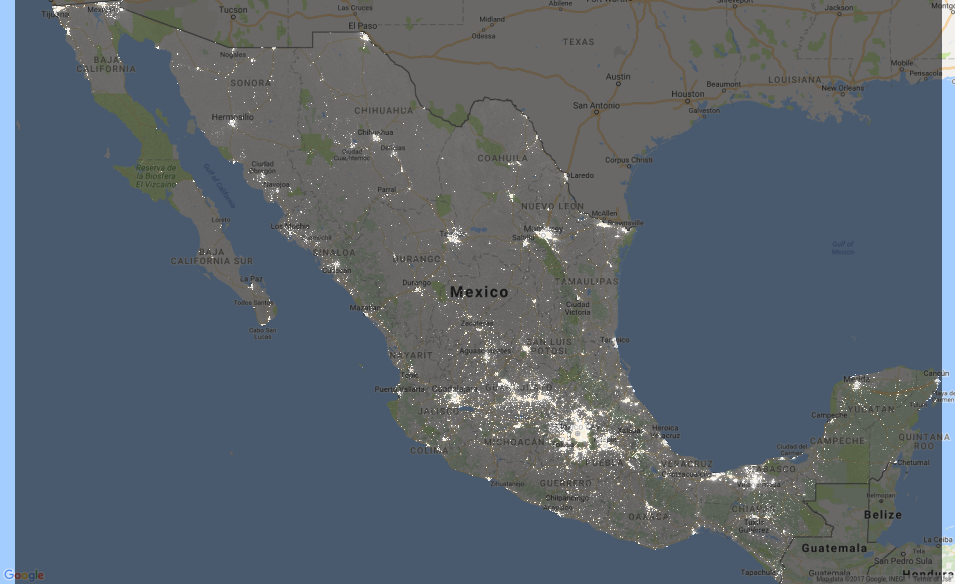
\includegraphics{../figures/mexico_viirs.png}
\caption{Foto satelital}
\end{figure}

Las fotos que se utilizaron son generadas con tecnología reciente que se
llama \emph{Suite de Radiometría de Imágenes Visibles Infrarojas},
VIIRS. Estas imágenes tienen una resolución de \(\text{0.55 km}^2\) y
usan unidades de radiación
\(\ell \sim \frac{\text{Watt}}{\text{cm}^2 \text{sr}}\), es decir
potencia entre área esférica. Llamaremos a estas mediciones como
\emph{luminosidad} y la denotamos como \(\ell\), \(\lambda\) o
\(\Lambda\), dependiendo del nivel y agregación.

Estas fuentes satelitales proporcionan mediciones geográficas
\(x_i,\, y_i\) y de luminosidad \(\ell_i\) que indexamos con
\(i \in \mathcal{I}\); las mediciones corresponden a los pixeles de la
cuadrícula o ráster. Relacionándolo con las regiones
\(R \in \mathcal{M},\, \mathcal{C},\, \mathcal{E}\) se tiene que el área
correspondiente es proporcional al número de pixeles contenidos en ellas
\[ \mathrm{A}(R) \propto \sum\limits_{i \in \mathcal{I}} \chi_R(x_i,y_i).\]

De forma similar calculamos la luminosidad total y media de las regiones
como
\[ \Lambda(R) = \sum\limits_{i \in \mathcal{I}} \ell_i \chi_R(x_i,y_i) \qquad y
      \qquad \lambda(R) = \frac{\Lambda(R)}{\mathrm{A}(R)}, \] donde
\(\chi_R(x_i,y_i)\) es la indicadora de cada pixel \(i\) en cada región
\(R\) de acuerdo a sus coordenadas \((x_i, y_i)\).

Mas aún dado que el índice medirá la actividad económica en las zonas
metropolitanas, se considera la luminosidad urbana como la restricción
de las luminosidades a las localidades urbanas. Tomamos
\(U = \bigcup_\mathcal{L}L\) como la unión de todas las localidades
urbanas, e indicamos mediante el superíndice \((\,\cdot\,)^U\) las
restricciones correspondientes
\[ \mathrm{A}^U(R) = \mathrm{A}(R \cap U), \qquad 
      \Lambda^U(R) = \Lambda(R \cap U), \qquad 
      \lambda^U(R) = \lambda(R \cap U). \]

Esta definición de localidad se aplica computacionalmente a partir de
los \emph{shapefiles} de localidades urbanas, cada cual pertenecen en sí
a un municipio, y por ende algunas a zonas metropolitanas y estados;
entonces las intersecciones se calculan en automático cuando se utiliza
este marco de localidades. Cabe mencionar que dichos \emph{shapefiles}
provienen del Marco Geoestadístico Nacional y se procesan con software
especializado\footnote{Se utiliza el sistema de información geográfica
  QGIS.} de geolocalización.

Finalmente se impone una segunda restricción a las zonas urbanas por
considerar. Esta restricción se basa en el valor de la luminosidad en la
fotografía, para que no exceda a
\(175\,\frac{\text{Watt}}{\text{cm}^2 \text{sr}}\). El límite se obtuvo
tras una inspección detallada, después de encontrar regiones de pocos
pixeles con luminosidades sumamente altas y que no corresponde a la
actividad. Más específicamente las zonas se identificaron en sitios de
actividad petrolera, como refinerías o extractoras, que inflarían la
luminosidad y por ende la actividad económica. El tope de 175 se toma
relativo al máximo de la Zona del Valle de México.

Manteniendo la notación simple, redefinimos la zona urbana \(U\) como no
petrolera donde solamente se consideran los pixeles con
\(\ell \leq 175\). La luminosidad correspondiente sigue esta
consideración.

Con estas medidas se calcularán los niveles del índice IMCO-OPI en las
zonas metropolitanas.

\subsection{Comisión Nacional Bancaria y de
Valores}\label{comision-nacional-bancaria-y-de-valores}

La CNBV proporciona datos mensuales de transacciones y otras variables
bancarias a nivel de localidad y por institución. Se utilizaron series
de transacciones en cajeros automáticos que denotamos como \(\mu\). Las
series más básicas llevan subíndices \(\mu_{m,t,b}\) y corresponden al
municipio \(m \in \mathcal{M}\), periodo \(t \in \mathcal{T}\) e
institución bancaria \(b \in \mathcal{B}\).

Las agrupaciones en cada índice se obtienen como sumas de los datos
individuales. En primer lugar se agregan las operaciones de cada
trimestre (con abuso de notación se utiliza el mismo subíndice \(t\));
en segundo lugar se distinguieron instituciones bancarias\footnote{Las
  observaciones de BBVA Bancomer y Santander fueron removidas de las
  sumas debido a volatilidad desproporcionada.} \(b \in \mathcal{B}\)
con observaciones volátiles y que tienen alta representación en el
total. Entonces consideramos un subconjunto de instituciones
\(\tilde{\mathcal{B}} \subset \mathcal{B}\) con respecto al cual
calculamos las series
\[ \mu_{m,t} = \sum_{b \in \tilde{\mathcal{B}}} \mu_{m,t,b}; \] a partir
de ellas se obtienen las series para las demás ciudades o estados
\(R \in \mathcal{C, E}\) \[ \mu_{R,t} = \sum_{m \subset R}\mu_{m,t}.\]

Por último, las series de transacciones de cajeros aproximan a la
actividad económica a través de los crecimientos proporcionales. Para
los periodos trimestral y anual --digamos \(p = 1,4\)-- denotamos dichos
crecimientos como\\
\[ \mu_{R,t}^{\Delta\,p} = \frac{\mu_{R,t}}{\mu_{R,t-p}} - 1.\]

A propósito de los índices en la notación, nótese que los subíndices
\(R,t\) corresponden a la medición en el espacio y tiempo, mientras que
los superíndices \(\Delta, p\) representan cuestiones estructurales de
los datos para el modelo.

\section{Modelado}\label{modelado}

La estrategia que sigue el desarrollo del índice metropolitano IMCO-OPI
consiste en entrenar un modelo a nivel estatal, para después replicarlo
con los datos correspondientes de las zonas metropolitanas. Denotamos
este índice de actividad económica como \(\varrho_{t}(R)\) y ajustamos a
diferentes regiones \(R \in \mathcal M, \mathcal E\), hacemos distinción
con el PIBE que mide el producto de los estados \(e \in \mathcal E\) y
se escribe como \(\pi_{e,t}\).

A su vez el modelo se separa en dos partes que corresponden al nivel y
al crecimiento. El cálculo de niveles se basa en los datos de
luminosidad urbana, mientras que el de crecimiento en los datos de
cajeros automáticos. Esta división apoya los siguientes puntos
considerables:

\begin{itemize}
\item
  La luminosidad refleja el tamaño de las economías. Artículos en la
  literatura como \emph{{[}1{]}, {[}2{]}} han apoyado esta tesis, y
  examinan características donde la relación se hace más o menos
  robusta.
\item
  Más específicamente, se asume que la actividad económica proviene de
  las localidades urbanas de las regiones. Esto se debe a que hay zonas
  oscuras que por su gran extensión acumulan luminosidad, pero que no es
  acorde con la producción debido a que está despoblada.
\item
  La actividad económica de las ciudades está ligada a las transacciones
  monetarias que hacen los consumidores, y más específicamente a las
  disposiciones en efectivo de las mismas. Este punto concuerda con el
  cálculo del ITAEE que incluye dichas transacciones, a la vez que se
  permite una agregación refinada.
\end{itemize}

La siguiente imagen resume la información de luminosidad y da muestra de
algunos elementos del modelo.

\begin{figure}[htbp]
\centering
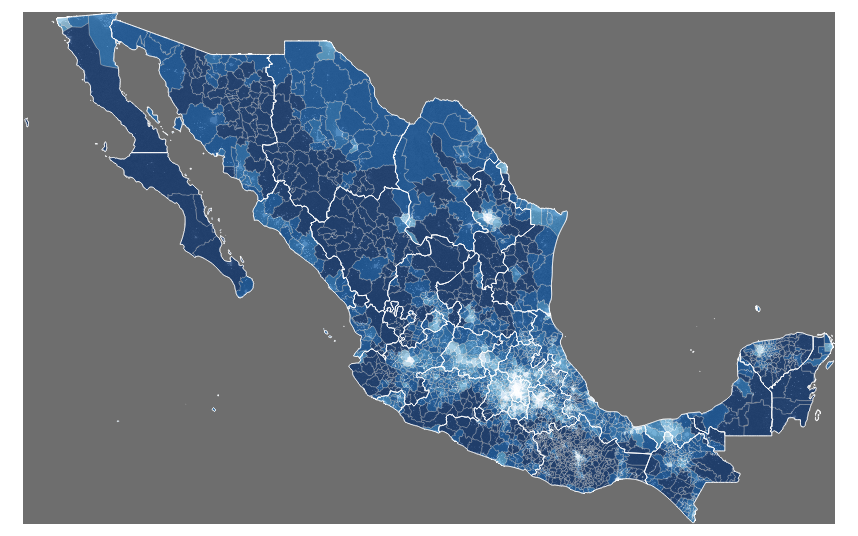
\includegraphics{../figures/municipios_viirs.png}
\caption{Luminosidad municipal}
\end{figure}

La intensidad del color de los municipios está relacionada con su
luminosidad logarítmica. Además se indican las fronteras de las
entidades federativas, a partir de la cual se estima el modelo.

En los siguientes apartados describimos los detalles técnicos.

\subsection{Niveles de actividad
económica}\label{niveles-de-actividad-economica}

Este cálculo utiliza los datos de PIBE de los estados y de luminosidad
urbana de los municipios. Para un tiempo inicial \(t_0 = 2014\), se
toman los datos correspondientes y se distribuye el PIBE con respecto a
la luminosidad. Para las ciudades o zonas metropolitanas, se agregan los
municipios correspondientes.

Para cada municipio \(m \in \mathcal M\) se calcula su actividad
económica como
\[ \mathrm{\varrho}_{t_0}(m) = \frac{\Lambda^{U}(m)}{\Lambda^{U}(e)} \pi_{e,t_0}\]
donde \(e = e(m)\) es el estado al que pertenece el municipio \(m\) y la
luminosidad \(\Lambda^U\) es la correspondiente a la luminosidad urbana
no petrolera --con \(\ell \leq 175\)-- que se introdujo anteriormente.

La actividad económica de las zonas metropolitanas \(c \in \mathcal C\),
se estima sumando sobre sus municipios
\[ \varrho_{t_0}(c)=\sum_{m \in c}\varrho_{t_0}(m).\] En el caso de las
metrópolis que se concentran en un sólo estado, esta estimación es igual
a la ponderación por luminosidad del PIBE correspondiente
\[ \varrho_{t_0}(c)=\frac{\Lambda^U(c)}{\Lambda^U(e)}\pi_{e,t_0}.\] Cabe
mencionar que éstas no son todas las zonas metropolitanas, pues hay
algunas que se dividen en dos o más entidades federativas. Éstas son
pocas por lo que podemos mencionarlas: La Laguna, La Piedad-Pénjamo,
Puebla-Tlaxcala, Puerto Vallarta y el Valle de México.

Si bien la representación en términos de sus municipios permite estimar
la actividad económica para estas zonas metropolitanas, también
controlamos por dicha separación a la vez que las representamos con sus
partes correspondientes, digamos \(c=c_1\cup c_2\) (\(\cup\ c_3\) para
el Valle de México) donde cada \(c_i\) pertenece a un estado diferente.

Después de considerar el nivel de actividad económica en \(t_0\), se
modela los niveles subsecuentes a partir del modelo de crecimiento de
las transacciones de cajeros automáticos que explicamos a continuación.

\subsection{Crecimiento}\label{crecimiento}

El crecimiento de actividad económica está ligado a los datos de
transacciones de cajeros automáticos. Esta consideración se puede
justificar tanto teóricamente como en la práctica si utilizamos el ITAEE
como el indicador base.

En la teoría, las transacciones de cajeros automáticos son una medida
simplifada del nivel de consumo en la sociedad, y éste tiene una
relación dinámica con la producción. En la práctica, el cálculo del
ITAEE utiliza datos de la banca comercial provistos por la
CNBV\footnote{Indicador Trimestral de la Actividad Económica Estatal.
  Fuentes y metodologías.}. En la gráfica \textbf{incluir gráfica} se ve
la similitud de las transacciones con la actividad económica que
representa el ITAEE en los estados.

Cuantificamos esta similitud con el siguiente modelo
\[ \iota_{e,t}^{\Delta,1} \sim \alpha_0^e + 
\alpha_1^e\mu_{e,t}^{\Delta,1} + \alpha_4\mu_{e,t}^{\Delta,4}\]

donde análogamente escribimos \((\,\cdot\,)^{\Delta,p}\) para los
crecimientos proporcionales trimestral y anual del ITAEE y las
transacciones de cajeros. Los coeficientes \(\alpha_{(\,\cdot\,)}^e\)
con superíndice están asociados a cada estado.

Los resultados de la estimación los expresamos con \(\hat \alpha\)'s
como coeficientes y \(\varepsilon\)'s como error
\[ \iota_{e,t}^{\Delta,1} = \hat\alpha_0^e + 
\hat\alpha_1^e\mu_{e,t}^{\Delta,1} + \hat\alpha_4\mu_{e,t}^{\Delta,4} + \varepsilon_{e,t}. \]

Estos modelos de crecimientos son los que aplicaremos a las zonas
metropolitanas, para después estimar los índices de las ciudades
\(\varrho_t(c)\).

\subsection{Integración de
crecimiento}\label{integracion-de-crecimiento}

Después de la estimación del crecimiento de los estados, se sigue
heredar la relación a las zonas metropolitanas que pertenecen a dichos
estados. Cambiando los datos observados en estados \(e\) por ciudades
\(c\) pero manteniendo los coeficientes nos queda,
\[ \varrho_{t}^{\Delta,1}(c) = \hat\alpha_0^e + 
\hat\alpha_1^e\mu_{c,t}^{\Delta,1} + \hat\alpha_4\mu_{c,t}^{\Delta,4} \]
donde \(e = e(c)\) es el estado al que pertenece la ciudad \(c\); o si
las ciudades pertenecen a más estados, se divide en las partes
correspondientes \(c=c_1\cup c_2\) (\(\cup\ c_3\) para el Valle de
México).

Junto con los niveles iniciales \(\varrho_{t_0}(c)\) podemos calcular
recursivamente las estimaciones de actividad económica en los diferentes
periodos del tiempo (antes y después),
\[ \varrho_{t-1}(c) = \frac{\varrho_t(c)}{1 + \varrho_t^{\Delta,1}(c)} \qquad
      \varrho_{t+1}(c) = \varrho_t(c)[1 + \varrho_t^{\Delta,1}(c)].\]

\section{Resultados}\label{resultados}

Incluimos las estimaciones de actividad económica de 2015.

\begin{table}[H]
\centering
\begingroup\scriptsize
\begin{tabular}{rlrrrr}
  \hline
 & Zona metropolitana & 201501 & 201504 & 201507 & 201510 \\ 
  \hline
1 & Acapulco & 97 816 & 97 131 & 97 630 & 102 529 \\ 
  2 & Aguascalientes & 167 784 & 170 912 & 169 888 & 175 806 \\ 
  3 & Campeche & 257 795 & 255 766 & 250 390 & 253 444 \\ 
  4 & Cancún & 153 612 & 156 000 & 158 145 & 163 084 \\ 
  5 & Cárdenas & 48 750 & 49 226 & 48 846 & 50 565 \\ 
  6 & Celaya & 88 777 & 90 653 & 90 239 & 94 552 \\ 
  7 & Chetumal & 27 500 & 27 875 & 28 346 & 29 488 \\ 
  8 & Chihuahua & 128 146 & 133 659 & 131 688 & 142 972 \\ 
  9 & Chilpancingo & 27 685 & 27 640 & 27 487 & 28 926 \\ 
  10 & Ciudad del Carmen & 208 707 & 211 041 & 205 925 & 208 591 \\ 
  11 & Ciudad Obregón & 48 219 & 49 766 & 49 039 & 52 445 \\ 
  12 & Ciudad Victoria & 33 651 & 33 378 & 33 806 & 33 791 \\ 
  13 & Coatzacoalcos & 125 620 & 125 984 & 125 559 & 127 703 \\ 
  14 & Colima-Villa de Álvarez & 50 184 & 50 568 & 50 716 & 52 051 \\ 
  15 & Córdoba & 23 286 & 23 419 & 23 335 & 23 786 \\ 
  16 & Cuautla & 52 369 & 53 115 & 52 483 & 55 371 \\ 
  17 & Cuernavaca & 94 259 & 94 260 & 94 252 & 98 541 \\ 
  18 & Culiacán & 124 406 & 127 249 & 120 280 & 136 128 \\ 
  19 & Durango & 65 136 & 65 617 & 66 357 & 68 437 \\ 
  20 & Ensenada & 49 431 & 50 937 & 50 625 & 53 373 \\ 
  21 & Guadalajara & 734 145 & 746 071 & 750 166 & 789 729 \\ 
  22 & Guanajuato & 22 968 & 23 534 & 23 477 & 24 204 \\ 
  23 & Guaymas & 34 079 & 34 149 & 32 907 & 35 442 \\ 
  24 & Hermosillo & 153 358 & 155 163 & 152 809 & 161 293 \\ 
  25 & Irapuato & 71 614 & 72 674 & 73 293 & 77 085 \\ 
  26 & Juárez & 213 013 & 228 766 & 229 145 & 248 785 \\ 
  27 & La Laguna & 270 345 & 271 785 & 273 312 & 282 462 \\ 
  28 & La Paz & 51 976 & 52 477 & 52 130 & 54 452 \\ 
  29 & La Piedad-Pénjamo & 25 800 & 25 972 & 25 787 & 26 901 \\ 
  30 & León & 220 765 & 226 290 & 227 475 & 240 800 \\ 
  31 & Los Cabos & 42 101 & 42 676 & 42 335 & 44 627 \\ 
  32 & Los Mochis & 46 004 & 47 615 & 46 539 & 51 641 \\ 
  33 & Manzanillo & 34 766 & 35 143 & 35 120 & 35 974 \\ 
  34 & Matamoros & 81 405 & 80 214 & 81 481 & 80 620 \\ 
  35 & Mazatlán & 70 644 & 72 724 & 71 980 & 79 426 \\ 
  36 & Mérida & 186 102 & 188 012 & 187 619 & 195 842 \\ 
  37 & Mexicali & 216 108 & 219 160 & 217 995 & 225 854 \\ 
  38 & Minatitlán & 86 931 & 87 713 & 87 437 & 89 030 \\ 
  39 & Monclova-Frontera & 67 409 & 69 846 & 69 583 & 71 628 \\ 
  40 & Monterrey & 1 036 203 & 1 056 433 & 1 063 692 & 1 108 417 \\ 
  41 & Morelia & 105 320 & 104 404 & 105 168 & 108 589 \\ 
  42 & Moroleón-Uriangato & 9 984 & 10 286 & 10 519 & 11 553 \\ 
  43 & Nuevo Laredo & 109 135 & 107 687 & 109 463 & 107 711 \\ 
  44 & Oaxaca & 78 230 & 78 796 & 79 247 & 82 351 \\ 
  45 & Ocotlán & 13 344 & 13 650 & 13 458 & 14 332 \\ 
  46 & Orizaba & 62 718 & 63 247 & 63 378 & 64 524 \\ 
  47 & Pachuca & 74 918 & 75 963 & 75 732 & 81 899 \\ 
  48 & Piedras Negras & 43 295 & 44 292 & 44 465 & 46 069 \\ 
  49 & Poza Rica & 54 002 & 54 534 & 54 166 & 55 132 \\ 
  50 & Puebla-Tlaxcala & 337 154 & 341 391 & 340 737 & 356 321 \\ 
  51 & Puerto Vallarta & 60 214 & 57 293 & 56 672 & 60 673 \\ 
  52 & Querétaro & 264 959 & 270 586 & 273 661 & 281 105 \\ 
  53 & Reynosa-Río Bravo & 156 556 & 153 401 & 154 621 & 153 553 \\ 
  54 & Rioverde-Ciudad Fernández & 9 122 & 9 173 & 9 144 & 9 502 \\ 
  55 & Salamanca & 50 172 & 51 836 & 51 927 & 54 474 \\ 
  56 & Saltillo & 139 744 & 143 441 & 144 503 & 149 230 \\ 
  57 & San Francisco del Rincón & 22 463 & 22 631 & 22 989 & 24 062 \\ 
  58 & San Juan del Río & 45 396 & 46 553 & 46 975 & 48 499 \\ 
  59 & San Luis Potosí-Soledad & 199 534 & 203 001 & 199 688 & 211 884 \\ 
  60 & Tampico-Pánuco & 98 493 & 98 214 & 99 719 & 98 410 \\ 
  61 & Tapachula & 21 207 & 20 984 & 21 059 & 21 776 \\ 
  62 & Tecomán & 11 692 & 11 933 & 11 919 & 12 330 \\ 
  63 & Tehuacán & 27 104 & 28 426 & 28 711 & 29 836 \\ 
  64 & Tehuantepec-Salina Cruz & 35 725 & 36 319 & 35 840 & 36 905 \\ 
  65 & Tepic & 56 434 & 56 726 & 56 197 & 58 320 \\ 
  66 & Tijuana & 166 201 & 172 950 & 174 612 & 184 189 \\ 
  67 & Tlaxcala-Apizaco & 45 704 & 47 848 & 48 571 & 52 476 \\ 
  68 & Toluca & 202 462 & 204 265 & 203 619 & 211 742 \\ 
  69 & Tula & 43 599 & 45 141 & 44 799 & 48 538 \\ 
  70 & Tulancingo & 21 641 & 22 139 & 22 224 & 23 876 \\ 
  71 & Tuxtla Gutiérrez & 99 355 & 100 622 & 100 222 & 103 750 \\ 
  72 & Uruapan & 32 495 & 32 487 & 32 530 & 33 582 \\ 
  73 & Valle de México & 3 721 558 & 3 770 848 & 3 752 562 & 3 977 424 \\ 
  74 & Veracruz & 161 464 & 163 347 & 162 807 & 165 297 \\ 
  75 & Villahermosa & 215 298 & 217 081 & 217 569 & 222 081 \\ 
  76 & Xalapa & 80 185 & 80 838 & 80 554 & 81 689 \\ 
  77 & Zacatecas-Guadalupe & 49 036 & 50 670 & 49 687 & 51 637 \\ 
  78 & Zamora-Jacona & 22 159 & 22 086 & 21 655 & 22 311 \\ 
   \hline
\end{tabular}
\endgroup
\end{table}


\end{document}
